\chapter{Best of Both Worlds}
\label{chap:best-of-both-worlds}
	In this chapter we present a framework for the transformation between the relational and document models.  The first component of this framework, detailed in \cref{sec:named-tuples-documents}, involves the encoding of named tuples into documents.  In \cref{sec:mapping-entity-groups-to-documents} we demonstrate the mapping of entity groups to documents.  In \cref{sec:encoding-entity-group-as-document-group} we show how to construct documents that encode the relations between tuples in the document model, preserving information that is otherwise lost during the transformation.
	
	We further demonstrate how to perform iterative search using these document encodings.
	
	\section{Encoding Named Tuples into Documents}
	\label{sec:named-tuples-documents}
		Recall in the extended document model (\cref{sec:extending-the-document-model}), a document \(\doc\) consists of fields \(\field_1, \field_2, \dotsc, \field_n\).  Using the extended document model, we are left with a straight forward mapping of a tuple \(\tuple\) to document \(\doc\).
		
		For tuple \(\tuple\), every attribute \(\attribute \in \attributes{\tuple}\) maps to a field \(\field\) in document \(\doc\).	Every attribute value is analyzed into an indexable form before being stored in a field.
		\begin{align}
			\attributes{\tuple} &\xrightarrow{analyzed} \fields{\doc} \\
			\attribute_1, \attribute_2, \dotsc, \attribute_n &\xrightarrow{analyzed} \field_1, \field_2, \dotsc, \field_n
		\end{align}
		
		We denote the document encoding of \(\tuple\) as \(\docs{\tuple}\).
		
		\begin{ex}
			Given the tuple
			\[
				\tuple = \{\text{code}: \text{``CDPS 101''}, \text{title}: \text{``Human-Mutant Relations''}, \text{subject}: \text{``CDPS''}\}
			\]
			
			we produce the document encoding \(\docs{\tuple}\) in \cref{tbl:docs-tuple}.
			
			\begin{table}
				\centering
				
				\begin{tabular}{ll}
					\toprule
					Field & Terms \\
					\midrule
					code & \(\{\text{cdps}, \text{101}\}\) \\
					title & \(\{\text{human}, \text{mutant}, \text{relations}\}\) \\
					subject & \(\{\text{cdps}\}\) \\
					\bottomrule
				\end{tabular}
				
				\caption{\(\docs{\tuple}\)}
				\label{tbl:docs-tuple}
			\end{table}
		\end{ex}

	
	\section{Mapping of Entity Groups to Documents}
	\label{sec:mapping-entity-groups-to-documents}
		Recall that an entity group (\cref{def:entity-group}) is a forest \(\egraph\) of tuples \(\tuple\) such that for every \((\tuple, \tuple') \in \egraph\), where \(\tuple \nequal \tuple'\), implies \(\relations{\tuple} \nequal \relations{\tuple'}\).  That is, every distinct tuple is from a distinct relation.
		
		Given the restriction
		\[
			\forall (\relation, \relation') \in \sgraph, \exists! (\relation, \relation') \models \theta
		\]
		
		we assert that if \(\tuple\) and \(\tuple'\) are in the entity group \(\egraph\), then there is a foreign key constraint between \(\tuple\) and \(\tuple'\).  We denote the vertices of \(\egraph\) as \(\text{V}(\egraph)\), and the edges of \(\egraph\) as \(\text{E}(\egraph)\).
		
		\begin{claim}
		\label{clm:lossless}
			Given \(\text{V}(\egraph)\), we are always able to reconstruct \(\egraph\).
		\end{claim}
		
		\begin{proof}
			Given \(\text{V}(\egraph)\), we must reconstruct \(\text{E}(\egraph)\) to complete \(\egraph\).
			
			Choose any \((\tuple, \tuple') \in \text{V}(\egraph)\).	If \((\relations{\tuple}, \relations{\tuple'}) \in \sgraph{\db}\), then \((\tuple, \tuple')\) is an edge in \(\egraph\).
			
			Recall our earlier assertion that \(\sgraph{\db}\) is cycle-free and foreign keys must be unique.
		\end{proof}
		
	\section{Encoding an Entity Group as a Document Group}
	\label{sec:encoding-entity-group-as-document-group}
		Given an entity group \(\egraph\), we construct two or more documents to represent the entity group in the document model.
		
		For every \(\tuple \in \text{V}(\egraph)\), we construct a document \(\docs{\tuple}\).  We construct an additional document, called the indexing document, which is the concatenation of all unique identifiers for every tuple in \(\text{V}(\egraph)\).
		
		Let \(x\) be the indexing document of \(\egraph\).
		\begin{align}
			x[\text{``entities''}] = \bigcup_{\tuple \in \text{V}\left(\egraph\right)} \uid{\tuple}
		\end{align}
		
		The encoding of \(\egraph\) is defined as the union of the set of documents for each tuple in \(\egraph\) and the indexing document, \(x\).
		\begin{align}
			\egraph \xrightarrow{\text{encode}} \{\docs{\tuple} : \tuple \in \text{V}(\egraph)\} \cup \{x\}
		\end{align}
		
		\begin{ex}
			An entity group produced from the schema in \cref{fig:schema-graph} is shown in \cref{fig:entity-group}.  Further transforming this entity group produces the documents in \cref{tbl:document-encoding}.
			
			\begin{figure}
				\centering
				
				\begin{dot2tex}[dot]
					digraph G {
						node [shape=plaintext]; {node [label="Course(MATH 360, Complex Analysis, MATH)"] course;}
						node [shape=plaintext]; {node [label="Subject(MATH, Mathematics)"] subject;}
						
						course -> subject;
					}
				\end{dot2tex}
				
				\caption{Example entity group}
				\label{fig:entity-group}
			\end{figure}
			
			\begin{table}
				\begin{subtable}[b]{0.33\linewidth}
					\centering
					
					\begin{tabular}{ll}
						\toprule
						Field & Terms \\
						\midrule
						\_\_id\_\_ & \(\{\text{subject|math\_360}\}\) \\
						code & \(\{\text{math}, \text{360}\}\) \\
						title & \(\{\text{complex}, \text{analysis}\}\) \\
						subject & \(\{\text{math}\}\) \\
						\bottomrule
					\end{tabular}
					
					\caption{Course}
				\end{subtable}
				\begin{subtable}[b]{0.33\linewidth}
					\centering
					
					\begin{tabular}{ll}
						\toprule
						Field & Terms \\
						\midrule
						\_\_id\_\_ & \(\{\text{subject|math}\}\) \\
						id & \(\{\text{math}\}\) \\
						name & \(\{\text{mathematics}\}\) \\
						\bottomrule
					\end{tabular}
					
					\caption{Subject}
				\end{subtable}
				\begin{subtable}[b]{0.33\linewidth}
					\centering
					
					\begin{tabular}{ll}
						\toprule
						Field & Terms \\
						\midrule
						entities & \(\{\text{course|math\_360}\), \\
						& \(\text{subject|math}\}\) \\
						\bottomrule
					\end{tabular}
					
					\caption{Indexing document}
				\end{subtable}
				
				\caption{Document encoding of \cref{fig:entity-group}}
				\label{tbl:document-encoding}
			\end{table}
		\end{ex}
		
		By \cref{clm:lossless}, we see that from \(\text{encode}(\egraph)\) we can recover \(\text{V}(\egraph)\), the tuples in \(\egraph\).
	
	\section{Encoding Attribute Values into Searchable Documents}
		Each value for user selected attributes are converted into \(n\)-grams, and stored in special documents.  These value documents permit users to perform fuzzy search for attributes, allowing attributes to be located despite character substitutions.  While this is not strictly necessary for the use of the system, it may reduce user fatigue.
		
		\begin{table}
			\centering
			\begin{tabular}{ll}
				\toprule
				Field & Terms \\
				\midrule
				\_\_class\_\_ & courses|code \\
				value & \{biol, 1010u\} \\
				code & \{biol, 1010u\} \\
				\_\_all\_\_ & \{\$\$b, \$bi, bio, iol, ol\$, l\$\$, \$\$1, \$10, 101, 010, 10u, 0u\$, u\$\$\} \\
				\bottomrule
			\end{tabular}
			
			\caption{Document representing a value of class ``courses|code''}
			\label{tbl:value-document}
		\end{table}
		
		As shown in \cref{tbl:value-document}, a value document permits \(n\)-gram search over values while providing the original value.  The system uses the value of found value documents to search for entities based on attributes.
		
		These values are unique within the space of all attribute values of a specific class.  They are not guaranteed to be unique within the entire space of documents.  This allows the system to provide additional information to users.  Rather than searching for a value, they are able to search for both a value and entity class.
	
	\section{Iterative Search Using Document Encodings}
		A document database supports fast and flexible keyword search queries.	A search query is characterized by \(\q = (\field, \w)\), where \(\field\) is an optional field name, and \(\w\) is a search phrase.
		
		\(\query(\q)\) is the set of documents returned by the text index.  The query function, combined with the extended document model, permits powerful search queries to be issued.  Our implementation supports approximate string matching using \(n\)-grams (\cref{sec:n-gram}) for values, searching for entities containing keywords (see \cref{ex:entity-search}), and the discovery of intermediate entities given two known entities.
		
		\begin{ex}[Entity Search]
		\label{ex:entity-search}
			Find all entities that match the keyword ``math''.
			
			Let \(\q = \text{``math''}\) be the search query.  The results are
			\begin{align*}
				\query(\q) &= \query(\text{``math''}) \\
				&= \{\text{subject|math}, \text{course|math\_360}\}
			\end{align*}
			
			which are coincidentally related.  The results of an entity search query are not necessarily related.
		\end{ex}
		
		\begin{ex}[Entity Graph Search]
			Find the shortest path between the two entities with the unique identities of ``subject|math'' and ``instructor|5''.
			
			The entity graph is shown in \cref{fig:path-initial}.  There are two possible paths between ``subject|math'' and ``instructor|5''.  The path in \cref{fig:path-2} is shorter than that in \cref{fig:path-1}, meaning it is likely the most relevant.
			
			\begin{figure}
				\centering
				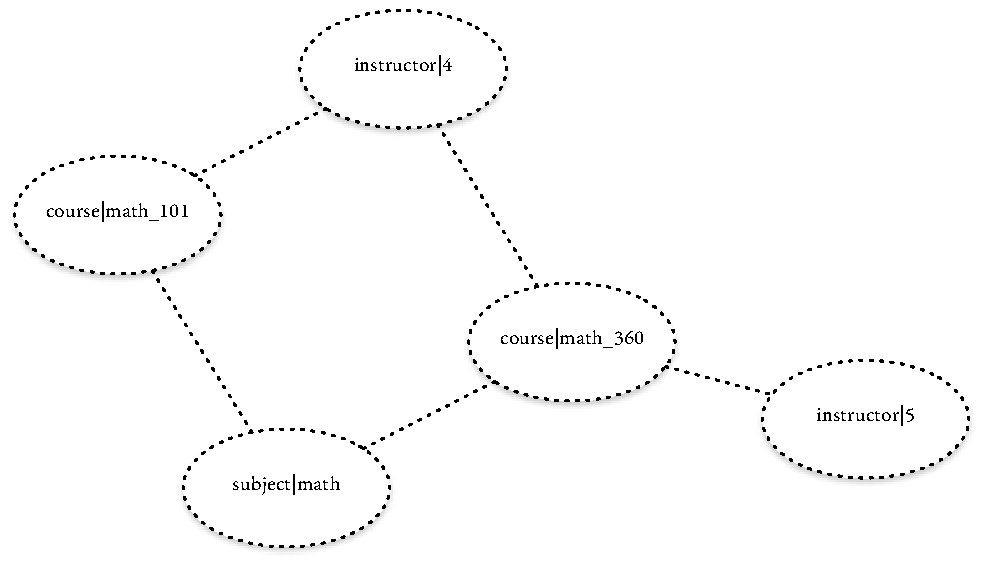
\includegraphics[scale=0.9]{figures/graphs/path/instructor-to-course-initial}
				
				\caption{Initial graph}
				\label{fig:path-initial}
			\end{figure}
			
			\begin{figure}
				\begin{subfigure}[b]{1.0\linewidth}
					\centering
					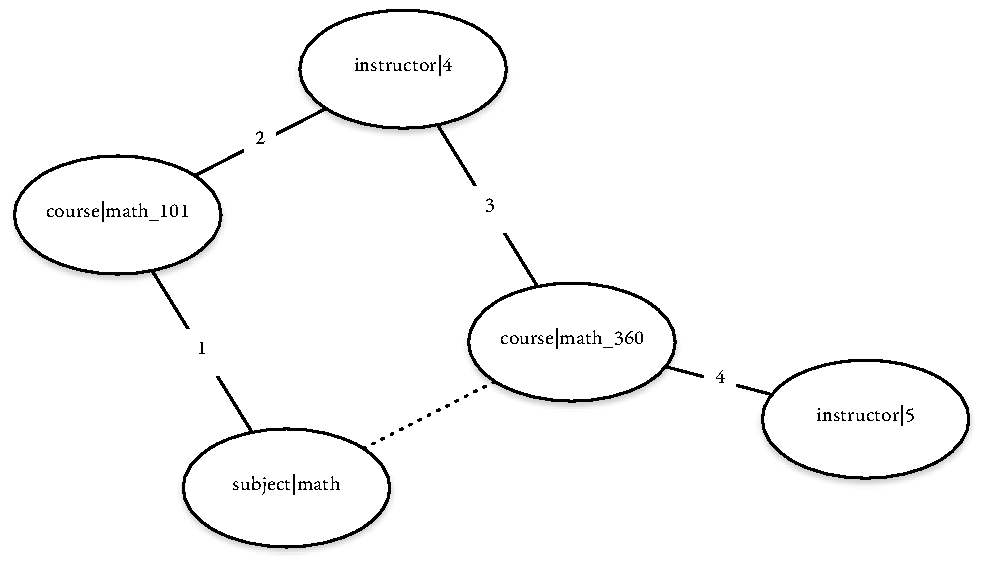
\includegraphics[scale=0.9]{figures/graphs/path/instructor-to-course-path-1}
					
					\caption{Valid path between two entities}
					\label{fig:path-1}
				\end{subfigure}
				\begin{subfigure}[b]{1.0\linewidth}
					\centering
					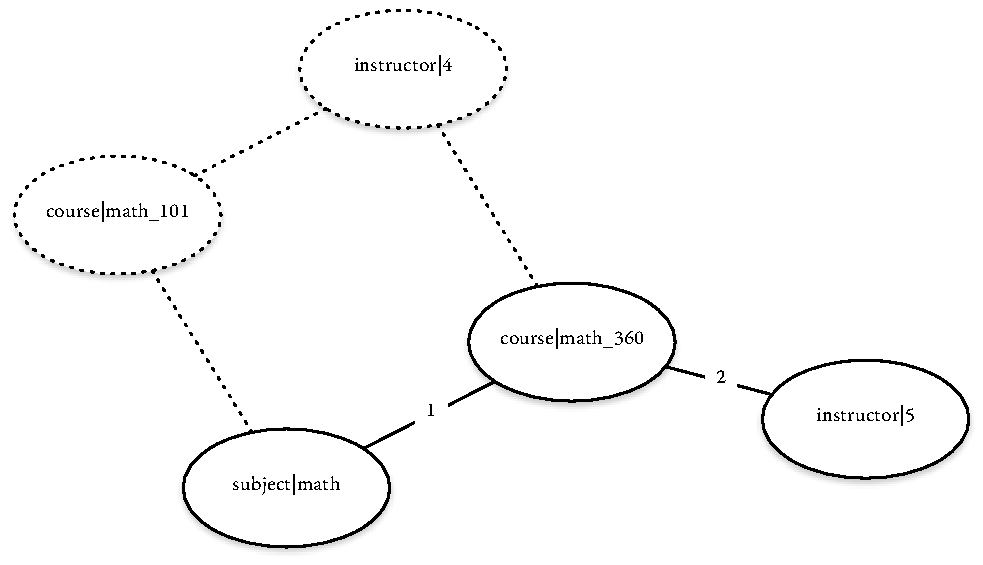
\includegraphics[scale=0.9]{figures/graphs/path/instructor-to-course-path-2}
					
					\caption{Shortest valid path between two entities}
					\label{fig:path-2}
				\end{subfigure}
				
				\caption{Two possible paths between ``subject|math'' and ``instructor|5''}
				\label{fig:paths}
			\end{figure}
		\end{ex}
		
		
		
		
		
		
		
		
		
		
		
		
		
		